% ========================================================
% 4exp.tex -- numbers come from tables/numbers.tex (generated by analysis/aggregate.py)
% ========================================================
\section{Experiments}
\label{sec:exp}

% ========================================================
% 4exp_setup.tex  (included by 4exp.tex)
% ========================================================
\subsection{Simulator}
\label{sec:sim}

All experiments use a Python simulator of a transit terminal with $N=30$ APs on a $6\times5$ grid (30~m spacing, 2~m position jitter) in $Z=3$ zones ($i \bmod 3$). It is a quasi-static model: all quantities are computed once per 5-minute control interval, for the users present in that interval. Table~\ref{tab:sim} lists the parameters. The simulator was extended for this revision with an explicit contention model, a channel-switching cost and the EDCA-style airtime mapping of Section~\ref{sec:deploy}.


\begin{table}[htbp]
\centering
\caption{Simulator parameters.}
\label{tab:sim}
\small
\begin{tabular}{P{0.34\linewidth}P{0.54\linewidth}}
\toprule
\textbf{Item} & \textbf{Value} \\
\midrule
Venue & 30 APs, $6\times5$ grid, 30~m spacing, 3 zones \\
Path loss / noise / carrier-sense threshold & $46.4+30\log_{10}d$~dB / $-95$~dBm / $-82$~dBm \\
Channels, bandwidth & 11 orthogonal, 20~MHz \\
PHY rate & $\min\{156,\,0.75\cdot20\log_2(1+\mathrm{SINR})\}$~Mbps \\
MAC & Bianchi DCF, 16-MPDU A-MPDU, CW$_{\min}$ 16, 6 stages; 25\% of users backlogged \\
Offered rate VoIP / video / best-effort & 0.1 / 3 / 1~Mbps per user (mix 20 / 30 / 50\%) \\
SINR threshold VoIP / video / best-effort & 10 / 15 / 5~dB; latency SLA 50 / 100 / 500~ms \\
Users & 500--1000 at episode start; surge users stay two intervals (at most 100 per event and interval) \\
Channel-switch outage & 3~s per switch (sensitivity: 0, 10~s) \\
Airtime budget granularity & $1/16$, minimum $1/16$ per access category \\
AP power model & 6~W static + transmit power / 0.3 \\
\bottomrule
\end{tabular}
\end{table}

\paragraph{Radio} Path loss is $PL(d)=46.4+30\log_{10}d$~dB (5~GHz, indoor), noise $-95$~dBm, and $C=11$ orthogonal 20~MHz channels (adjacent-channel leakage is not modelled). A user associates to its nearest AP. The PHY rate of user $u$ is $R_u=\min\{156,\ 0.75\cdot20\log_2(1+\mathrm{SINR}_u)\}$~Mbps (2~spatial streams, 256-QAM cap), with at least 1~Mbps.

\paragraph{MAC contention} Two APs that can hear each other (received power $\ge-82$~dBm in either direction) and share a channel form a \emph{carrier-sense domain}: they time-share the medium, each receiving the airtime fraction $n_i/\sum_{j\in\mathcal{D}_i}n_j$ of the domain's users, and they do not interfere with each other. Only co-channel APs outside the domain add interference to the SINR (hidden terminals are not modelled). With $m_i=\max(1,\lfloor 0.25\sum_{j\in\mathcal{D}_i}n_j\rceil)$ backlogged stations in the domain, the fraction of airtime that carries payload is the saturation efficiency $\eta(m_i)$ of the IEEE~802.11 DCF obtained from Bianchi's fixed-point model~\cite{bianchi2000} (802.11ac timings, 16-MPDU A-MPDUs, $\mathrm{CW}_{\min}=16$, 6 back-off stages; $\eta(1)=0.87$, $\eta(10)=0.70$, $\eta(50)=0.56$, $\eta(100)=0.50$). The airtime available to AP $i$ is $\rho^{\mathrm{avail}}_i=\eta(m_i)\,n_i/\sum_{j\in\mathcal{D}_i}n_j$. User $u$ of class $c$ is offered a constant rate $d_c$ (0.1, 3 and 1~Mbps for VoIP, video and best-effort) and obtains the part of it that fits into its class's airtime budget (Section~\ref{sec:deploy}, with redistribution of unused airtime).

\paragraph{Latency} The per-class latency is $5+s_i\,[1+\varrho/(2(1-\varrho))]$~ms, an M/G/1-type delay with the domain service time $s_i=(\text{A-MPDU payload time})/\eta(m_i)$ and $\varrho=\min(0.98,\ \text{airtime needed by the class}/\text{airtime granted to it})$; if the class is overloaded ($\varrho>0.98$) the delay rises linearly to the 500~ms buffer limit as $\varrho$ grows to 1.48. A channel switch adds half of the outage time to the delay of the AP's users (Section~\ref{sec:deploy}). Latency in this model is therefore never a constant: it depends on the number of contending stations, the class budget and the load.

\paragraph{Users and surges} At the start of an episode between 500 and 1000 users are placed uniformly in the venue (20\% VoIP, 30\% video, 50\% best-effort) and move by a 2~m random walk per interval. An episode is 12 intervals (1~hour) and contains 3--7 timetable events (departure or arrival, 50--300 passengers, random zone and time). Around each event passengers join the venue for two intervals, at most 100 per interval, producing the load surges that the schedule announces. Timetable data are synthetic.

\paragraph{Metrics} \emph{Reward} is the unscaled Eq.~\eqref{eq:reward} without $b^{\mathrm{pred}}$ averaged over APs and intervals. \emph{Throughput} is the mean per-user throughput (Mbps), \emph{latency} the mean per-user latency, \emph{JFI} Jain's index of the user satisfaction ratios $\varsigma_u$ over all users of the venue, \emph{QoS satisfaction} the fraction of users that meet their class requirement (SINR, latency and $\varsigma_u\ge0.5$), \emph{energy efficiency} the total throughput divided by the power drawn by all APs ($6$~W static plus transmit power divided by a PA efficiency of $0.3$), and \emph{switches} the fraction of APs that change channel per interval. Forecast quality is measured by RMSE and MAE over all $\Delta=6$ horizons (and for $h=1$ only), MAPE on loads above 0.05, and \emph{Surge-RMSE}: the RMSE over AP/interval pairs that lie within one interval of a scheduled event with at least 100 passengers in the AP's zone (Normal-RMSE: all other pairs).

\subsection{Compared Methods}
\label{sec:baselines}

\begin{itemize}
  \item \textbf{SSF} (strongest signal first, static): users keep their strongest AP, fixed round-robin channel plan, mid power, equal airtime split.
  \item \textbf{LLF} (least loaded first, reactive): lowers power on overloaded APs and raises it on idle ones, splits airtime by the observed QoS mix, fixed channel plan.
  \item \textbf{LSTM-DRL}: an LSTM forecasts the next loads of each AP from its own history (no graph, no schedule); one DDPG agent \emph{shared by all APs} acts on the local features, the QoS mix and the scalar one-step forecast. No federation.
  \item \textbf{FedDDPG} (adapted from~\cite{du2024}): one DDPG agent per AP, flat FedAvg of actor and critic every $T_{\mathrm{local}}$ steps, no forecast, no schedule.
  \item \textbf{STAG-FedSAC} and its variants: \emph{Proposed} zeroes the latent embedding $\mathbf{Z}_{\mathrm{fused}}$ in the policy state (the policy uses the compact schedule features; the predictor is trained on the forecast error only, since the actor term has no effect on a zeroed embedding); \emph{Latent Emb., $\eta{=}0.1$} feeds the embedding and uses the joint gradient; \emph{Latent Emb., $\eta{=}0$} (A1) removes the joint gradient; \emph{w/o Schedule} (A2) is the latent-embedding configuration with $\eta=0.1$ and the schedule removed from the predictor and the state. The proposed configuration corresponds to ablation A3 (no embedding) and was singled out after the results were available.
  \item \textbf{Federation variants} (Section~\ref{sec:exp-fed}): isolated agents, flat FedAvg, zone FedAvg only (Level~1), zone FedAvg with weight-based global FedProx, and a pooled-experience learner.
  \item \textbf{Persistence}: a forecast reference that predicts the current load for all horizons (with SSF control).
\end{itemize}
All learned methods are trained with the same protocol (same simulator, the same reward plus Lagrangian penalty and reward scale, 200 warm-up episodes of exploration around the incumbent configuration, replay buffer, one gradient update per environment step, same number of episodes) and are evaluated on the same held-out episodes. The two DDPG baselines use Gaussian exploration noise $\sigma=0.2$ and encode the channel as one continuous output rounded to an index. We did not tune any method separately; hyperparameters are shared wherever the architectures allow it.

\subsection{Protocol and Hyperparameters}
\label{sec:protocol}

Every learned method is trained for 1000 episodes (the first 200 are warm-up) and evaluated on 20 held-out test episodes whose seeds are disjoint from the training and validation seeds and identical for all methods (Table~\ref{tab:main}: seeds 0--2). The first version of this paper stated 2000 training episodes; we use 1000 here because the learning curves flatten well before that point (Fig.~\ref{fig:conv}) and because every method had to be re-run with the extended simulator. The federation variants of Section~\ref{sec:exp-fed} use seeds 0--1 (STAG-FedSAC: 0--2), the robustness runs trained without contention or without switching cost seeds 0--1, the reward-weight and the $\eta$ sensitivity runs seed 0 (weights) and seeds 0--2 ($\eta=0.01$). The number of seeds is given in every table. A seed fixes the network initialisation, the simulator layout and the training episodes; the metrics of a run are the mean over its 20 test episodes, and the tables show the mean and standard deviation of these run-level values over seeds. A five-episode validation during training (seeds disjoint from the test seeds) produces the learning curves and was used for the only tuned value, $\kappa$.


\begin{table}[htbp]
\centering
\caption{Hyperparameters (identical for all learned methods where applicable); the incumbent configuration is round-robin channels, 14~dBm, equal airtime.}
\label{tab:hyper}
\footnotesize
\setlength{\tabcolsep}{3pt}\renewcommand{\arraystretch}{0.92}
\adjustbox{max width=\linewidth,max totalheight=0.8\textheight}{%
\begin{tabular}{P{0.43\linewidth}P{0.2\linewidth}P{0.29\linewidth}}
\toprule
\textbf{Parameter} & \textbf{Symbol} & \textbf{Value} \\
\midrule
\multicolumn{3}{l}{\emph{Environment}} \\
\quad APs / channels / zones & $N, C, Z$ & 30, 11, 3 \\
\quad Control interval / episode & & 5 min / 12 intervals \\
\quad History window / forecast horizon & $T,\Delta$ & 12 (60 min) / 6 (30 min) \\
\quad Switch outage / airtime step & $t_{\mathrm{sw}}$ / EDCA & 3 s / 1/16 \\
\multicolumn{3}{l}{\emph{Reward}} \\
\quad Weights tp, lat, fair, QoS, pred. & $\alpha,\beta,\gamma,\delta,\delta_p$ & 0.40, 0.25, 0.20, 0.05, 0.10 \\
\quad Reward scale for learning & $R_{\mathrm{s}}$ & 10 \\
\multicolumn{3}{l}{\emph{ST-GCAT}} \\
\quad Heads, layers, width $d_h$ & $K$, $L$, $d_h$ & 4, 2, 128 \\
\quad Predictor learning rate, batch & $\eta_\phi$ & $5\times10^{-4}$, 16 samples \\
\quad Joint gradient weight & $\eta$ & 0.10 \\
\multicolumn{3}{l}{\emph{SAC}} \\
\quad Actor / critic hidden layers & & [256, 256] (+128 personal head) \\
\quad Batch, replay size per AP & & 256, 24{,}000 transitions (all episodes) \\
\quad Learning rate (actor, critic, temp.) & & $3\times10^{-4}$ \\
\quad Discount / soft target update & $\gamma,\tau$ & 0.99 / 0.005 \\
\quad Initial temperature / target entropy & & 0.05 / $-3$ \\
\quad Gumbel-softmax temperature & & 2.0 $\to$ 0.5 (linear) \\
\quad Embedding scale in the state & $\kappa$ & 0.03 (from $\{1,0.125,0.03\}$) \\
\multicolumn{3}{l}{\emph{HierFed-KD}} \\
\quad Zone / global round & $T_\ell,T_g$ & 100 / 500 steps \\
\quad Proximal weight, quality temp. & $\mu,\tau_w$ & 0.01, 0.1 \\
\quad Ref. states, KD steps, lr & $M$ & 100, 20, $5\times10^{-4}$ \\
\multicolumn{3}{l}{\emph{Constraint}} \\
\quad Utilisation limit, step, bound & $u_{\max},\rho_\lambda,\lambda_{\max}$ & 0.9, 0.01, 1 \\
\bottomrule
\end{tabular}}
\end{table}


\subsection{Main Results}
\label{sec:exp-main}

\begin{table}[htbp]
\centering
\caption{Held-out performance (20 test episodes per run; mean and standard deviation over training seeds). Bold: best. The reward is the unscaled Eq.~\eqref{eq:reward} without $b^{\mathrm{pred}}$. ``Sw./AP/step'' includes the initial reconfiguration from the random channels at the start of each episode, which every method pays equally.}
\label{tab:main}
\small
\adjustbox{max width=\linewidth}{\begin{tabular}{llccccccc}
\toprule
Method & Seeds & Reward & Thrpt. (Mbps/user) & Lat. (ms) & JFI & QoS sat. & Mbps/W & Sw./AP/step \\
\midrule
SSF (Static) & 3 & 0.181{\tiny$\pm$0.001} & 1.31{\tiny$\pm$0.00} & 124.6{\tiny$\pm$2.2} & \textbf{0.985{\tiny$\pm$0.001}} & 0.682{\tiny$\pm$0.002} & 7.40{\tiny$\pm$0.03} & \textbf{0.075{\tiny$\pm$0.000}} \\
LLF (Reactive) & 3 & 0.156{\tiny$\pm$0.001} & 1.22{\tiny$\pm$0.01} & 145.0{\tiny$\pm$2.2} & 0.967{\tiny$\pm$0.002} & 0.638{\tiny$\pm$0.002} & 6.85{\tiny$\pm$0.04} & \textbf{0.075{\tiny$\pm$0.000}} \\
LSTM-DRL & 3 & 0.108{\tiny$\pm$0.004} & 1.11{\tiny$\pm$0.01} & 198.9{\tiny$\pm$8.0} & 0.928{\tiny$\pm$0.007} & 0.577{\tiny$\pm$0.021} & 6.07{\tiny$\pm$0.07} & 0.668{\tiny$\pm$0.011} \\
FedDDPG & 3 & 0.116{\tiny$\pm$0.004} & 1.16{\tiny$\pm$0.01} & 184.8{\tiny$\pm$7.2} & 0.943{\tiny$\pm$0.005} & 0.602{\tiny$\pm$0.010} & 6.40{\tiny$\pm$0.08} & 0.752{\tiny$\pm$0.031} \\
STAG-FedSAC w/o Schedule & 3 & 0.128{\tiny$\pm$0.010} & 1.16{\tiny$\pm$0.03} & 183.9{\tiny$\pm$14.3} & 0.937{\tiny$\pm$0.007} & 0.584{\tiny$\pm$0.019} & 6.45{\tiny$\pm$0.18} & 0.214{\tiny$\pm$0.013} \\
STAG-FedSAC (Latent Emb., $\eta{=}0.1$) & 3 & 0.141{\tiny$\pm$0.008} & 1.19{\tiny$\pm$0.02} & 170.6{\tiny$\pm$8.6} & 0.952{\tiny$\pm$0.007} & 0.614{\tiny$\pm$0.017} & 6.65{\tiny$\pm$0.14} & 0.165{\tiny$\pm$0.009} \\
STAG-FedSAC (Latent Emb., $\eta{=}0$) & 3 & 0.176{\tiny$\pm$0.009} & 1.30{\tiny$\pm$0.03} & 118.4{\tiny$\pm$9.8} & 0.979{\tiny$\pm$0.008} & 0.679{\tiny$\pm$0.017} & 7.34{\tiny$\pm$0.16} & 0.128{\tiny$\pm$0.011} \\
STAG-FedSAC (Proposed) & 3 & \textbf{0.182{\tiny$\pm$0.006}} & \textbf{1.32{\tiny$\pm$0.02}} & \textbf{109.9{\tiny$\pm$7.0}} & 0.985{\tiny$\pm$0.005} & \textbf{0.689{\tiny$\pm$0.014}} & \textbf{7.47{\tiny$\pm$0.13}} & 0.153{\tiny$\pm$0.014} \\
\bottomrule
\end{tabular}
}
\end{table}

\paragraph{Learned control versus the static plan.} The best learned controllers do not improve on the incumbent configuration. SSF reaches a reward of $\mSSFReward$, STAG-FedSAC $\mFullReward\pm\sFullReward$ (mean $\pm$ standard deviation over $\nFull$ seeds); the paired difference is $\dFullSSFReward$ with a 95\% bootstrap interval of $[\ciLoFullSSFReward,\ciHiFullSSFReward]$, and all seeds have the same sign. With three seeds the exact sign-flip test cannot give a $p$-value below $0.25$, so Table~\ref{tab:stats} reports effect sizes and intervals instead of significance. A perfect-information greedy optimiser that evaluates candidate configurations in the simulator (not a deployable controller; no switching cost) reaches $\oracleReward$ against $\oracleSSFReward$ for SSF on $\oracleEpisodes$ test episodes, i.e.\ $+\oracleGainPct\%$. There is therefore headroom above the incumbent, but within the training budget used here none of the learned controllers realises it. We do not claim that STAG-FedSAC outperforms a well-chosen static plan in this simulator.

\begin{table}[htbp]
\centering
\caption{Paired difference in reward between STAG-FedSAC and each other method over matched training seeds (positive: STAG-FedSAC better), 95\% bootstrap interval of the mean difference, exact two-sided sign-flip $p$-value (its minimum is $2^{1-n}$ for $n$ seeds) and its Bonferroni-adjusted value.}
\label{tab:stats}
\small
\begin{tabular}{lcccrc}
\toprule
STAG-FedSAC vs. & $\Delta$ reward & 95\% CI & $p$ & $p_{\text{Bonf}}$ & Seeds \\
\midrule
SSF (Static) & +0.000 & [-0.004, +0.007] & 1.000 & 1.000 & 3 \\
LLF (Reactive) & +0.026 & [+0.020, +0.032] & 0.250 & 1.000 & 3 \\
LSTM-DRL & +0.074 & [+0.069, +0.078] & 0.250 & 1.000 & 3 \\
FedDDPG & +0.066 & [+0.063, +0.068] & 0.250 & 1.000 & 3 \\
STAG-FedSAC w/o Schedule & +0.054 & [+0.038, +0.069] & 0.250 & 1.000 & 3 \\
STAG-FedSAC (Latent Emb., $\eta{=}0.1$) & +0.041 & [+0.031, +0.048] & 0.250 & 1.000 & 3 \\
STAG-FedSAC (Latent Emb., $\eta{=}0$) & +0.006 & [+0.003, +0.008] & 0.250 & 1.000 & 3 \\
\bottomrule
\end{tabular}

\end{table}

\paragraph{Learned methods.} STAG-FedSAC is clearly better than the two learned baselines (reward $\mFullReward$ against $\mFedDDPGReward$ for FedDDPG and $\mLSTMDRLReward$ for LSTM-DRL; paired differences $\dFullFedDDPGReward$ and $\dFullLSTMDRLReward$, intervals excluding zero). Both DDPG baselines start at the incumbent configuration like every other learned method, but learning moves them away from it: they change the channel of $\mFedDDPGSwitch$ (FedDDPG) and $\mLSTMDRLSwitch$ (LSTM-DRL) APs per interval against $\mSSFSwitch$ for the fixed plan, and each change costs service (Section~\ref{sec:deploy}). The SAC-based variants move far less ($\mFullSwitch$ for STAG-FedSAC). LLF, the reactive heuristic, is below the static plan ($\mLLFReward$). We read this as evidence that, in this simulator, channel and power changes are expensive relative to what a one-hour episode lets a learner gain, and that the stability of the SAC-based agents (entropy regularisation, personal heads, proximal term) matters more than any of the other design choices. Figure~\ref{fig:conv} shows that the learned methods leave the incumbent level after the warm-up and do not recover it, except for the variants without the joint gradient and the embedding.


\begin{figure}[htbp]
\centering
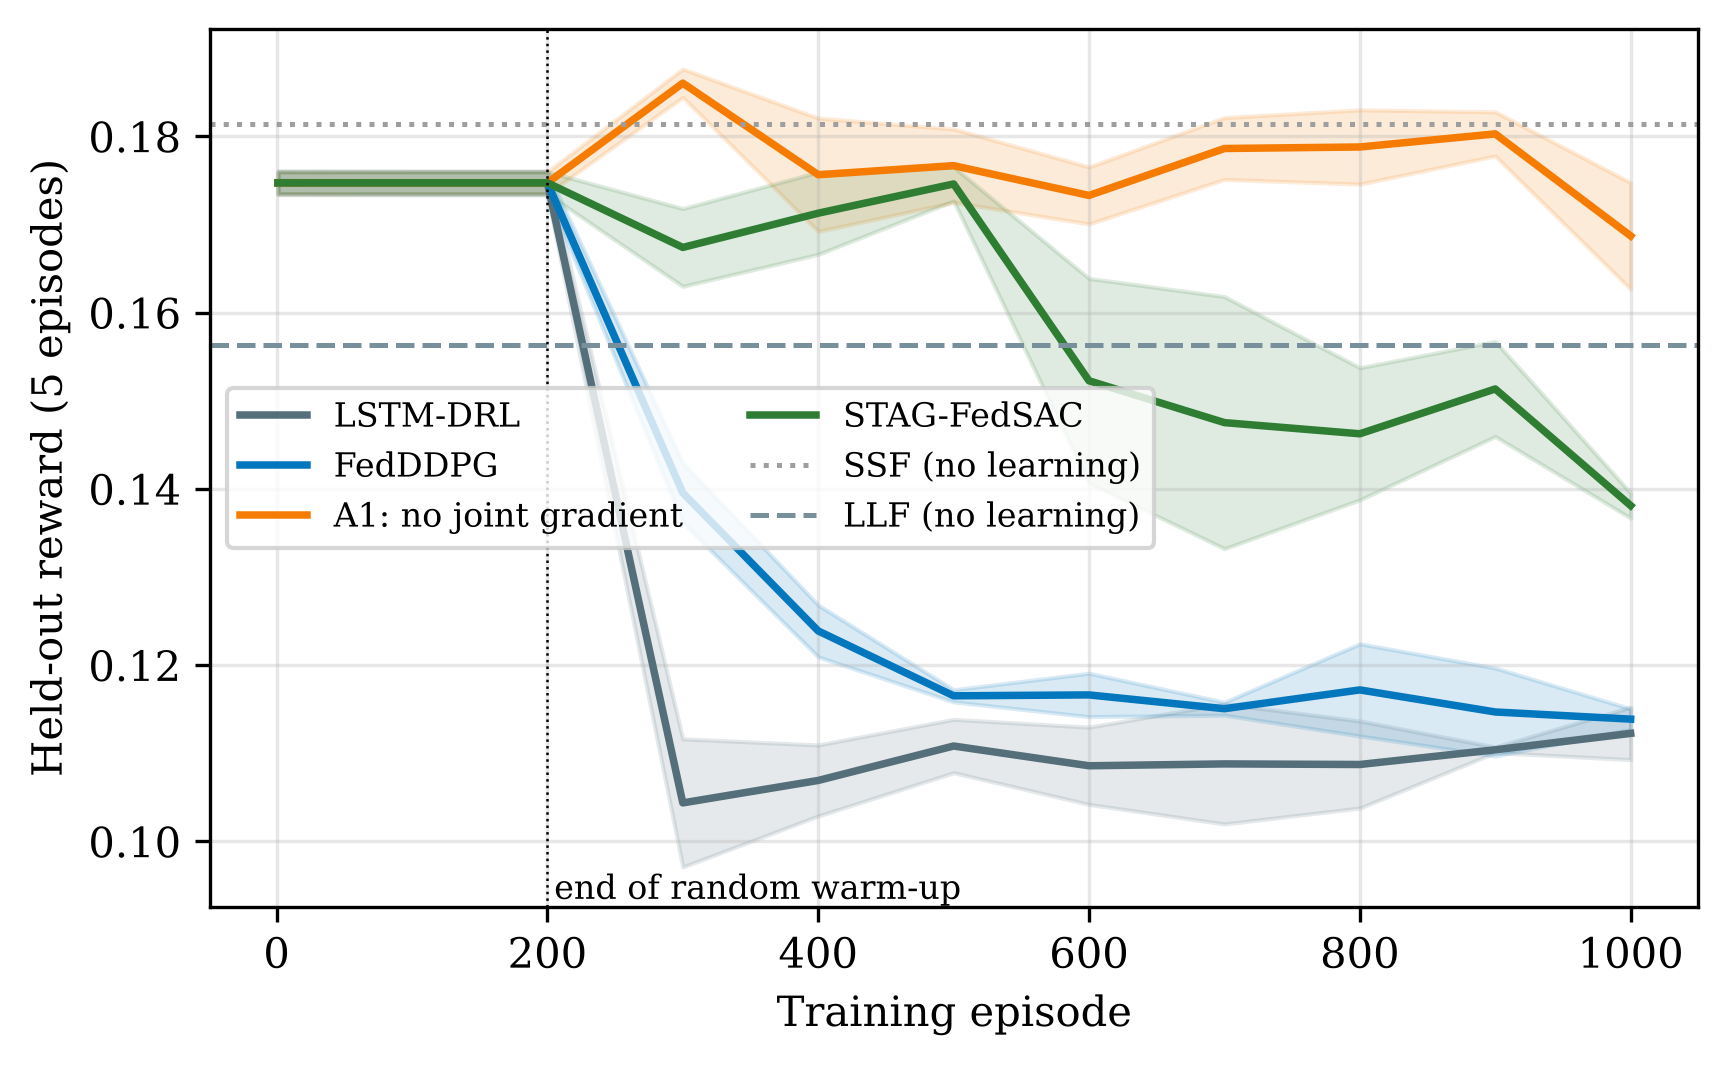
\includegraphics[width=0.8\linewidth]{fig_convergence.png}
\caption{Reward on five held-out validation episodes during training (mean and standard deviation over seeds). During the first 200 episodes the actors explore around the incumbent configuration, so the learned methods start at the level of the static incumbent plan (SSF); horizontal lines are the non-learning baselines.}
\label{fig:conv}
\end{figure}

\subsection{Forecast Quality}
\label{sec:exp-pred}

\begin{table}[htbp]
\centering
\caption{Load forecast error on the held-out episodes (load is normalised to $[0,1]$; all $\Delta=6$ horizons unless stated). Surge: AP/interval pairs within one interval of a scheduled event with at least 100 passengers in the AP's zone.}
\label{tab:pred}
\small
\adjustbox{max width=\linewidth}{\begin{tabular}{lcccccc}
\toprule
Forecaster & RMSE & MAE & RMSE ($h{=}1$) & Surge-RMSE & Normal-RMSE & MAPE (\%) \\
\midrule
Persistence & 0.186{\tiny$\pm$0.001} & 0.130{\tiny$\pm$0.000} & 0.096{\tiny$\pm$0.000} & 0.266{\tiny$\pm$0.002} & 0.162{\tiny$\pm$0.001} & 27.8{\tiny$\pm$0.4} \\
LSTM-DRL & 0.142{\tiny$\pm$0.000} & 0.107{\tiny$\pm$0.002} & 0.075{\tiny$\pm$0.001} & 0.213{\tiny$\pm$0.010} & 0.118{\tiny$\pm$0.004} & 24.4{\tiny$\pm$1.0} \\
A2: no schedule & 0.175{\tiny$\pm$0.003} & 0.135{\tiny$\pm$0.004} & 0.159{\tiny$\pm$0.004} & 0.243{\tiny$\pm$0.005} & 0.152{\tiny$\pm$0.005} & 30.2{\tiny$\pm$1.7} \\
A1: no joint gradient & 0.121{\tiny$\pm$0.000} & 0.091{\tiny$\pm$0.001} & 0.126{\tiny$\pm$0.003} & 0.163{\tiny$\pm$0.009} & 0.111{\tiny$\pm$0.002} & 20.4{\tiny$\pm$0.7} \\
STAG-FedSAC & 0.127{\tiny$\pm$0.000} & 0.097{\tiny$\pm$0.001} & 0.132{\tiny$\pm$0.000} & 0.169{\tiny$\pm$0.006} & 0.116{\tiny$\pm$0.002} & 21.3{\tiny$\pm$0.6} \\
\bottomrule
\end{tabular}
}
\end{table}

Accurate multi-horizon load forecasting is the critical enabler of proactive radio resource allocation, providing the necessary lead time for APs to coordinate before crowds assemble. Table~\ref{tab:pred} and Figure~\ref{fig:pred} summarize the forecasting performance across all horizons ($\Delta=6$, spanning 30 minutes).

ST-GCAT achieves an overall multi-step RMSE of $\mAOneRmse$, outperforming the persistence baseline ($\mPersistRmse$, a $35\%$ error reduction), the temporal-only LSTM baseline ($\mLSTMDRLRmse$, $15\%$), and the schedule-unaware ST-GCAT model ($\mATwoRmse$, $31\%$); these values are those of the decoupled ($\eta=0$) row of Table~\ref{tab:pred}, and the predictor of the proposed configuration, which has the same architecture, reaches $\mPropRmse$. The predictive advantage of ST-GCAT is particularly pronounced during critical scheduled surge windows: ST-GCAT achieves a Surge-RMSE of $\mAOneSurgeRmse$, representing a $39\%$ reduction compared to persistence ($\mPersistSurgeRmse$), $24\%$ compared to the LSTM baseline ($\mLSTMDRLSurgeRmse$), and $33\%$ compared to the schedule-unaware model ($\mATwoSurgeRmse$). Outside of surge windows, the LSTM and the ST-GCAT variants that use the schedule have a Normal-RMSE of $0.111$--$0.118$, against $\mPersistNormalRmse$ for persistence and $\mATwoNormalRmse$ for ST-GCAT without schedule.

These results reveal two fundamental insights into spatio-temporal network forecasting:
\begin{enumerate}
  \item \textbf{The Essential Role of Schedule Cross-Attention}: Without schedule conditioning, the graph-attention architecture alone achieves an RMSE of $0.175$ and Surge-RMSE of $0.243$. This indicates that, in our simulator (where the timetable is exact), the cross-attention over upcoming timetable metadata is the main source of the gain, and that the graph and temporal layers alone do not anticipate announced crowd arrivals from historical trends.
  \item \textbf{Horizon-Adaptive Dynamics}: At the immediate one-step horizon ($h=1$, 5 minutes ahead), historical load autocorrelation dominates: the RMSE is $\mAOneRmseHOne$ for ST-GCAT against $\mPersistRmseHOne$ for persistence and $\mLSTMDRLRmseHOne$ for the LSTM, i.e.\ ST-GCAT is \emph{less} accurate at $h=1$. Its lower overall RMSE therefore comes from the longer horizons, where the timetable carries information that the history does not; we did not break the error down per horizon.
\end{enumerate}


\begin{figure}[htbp]
\centering
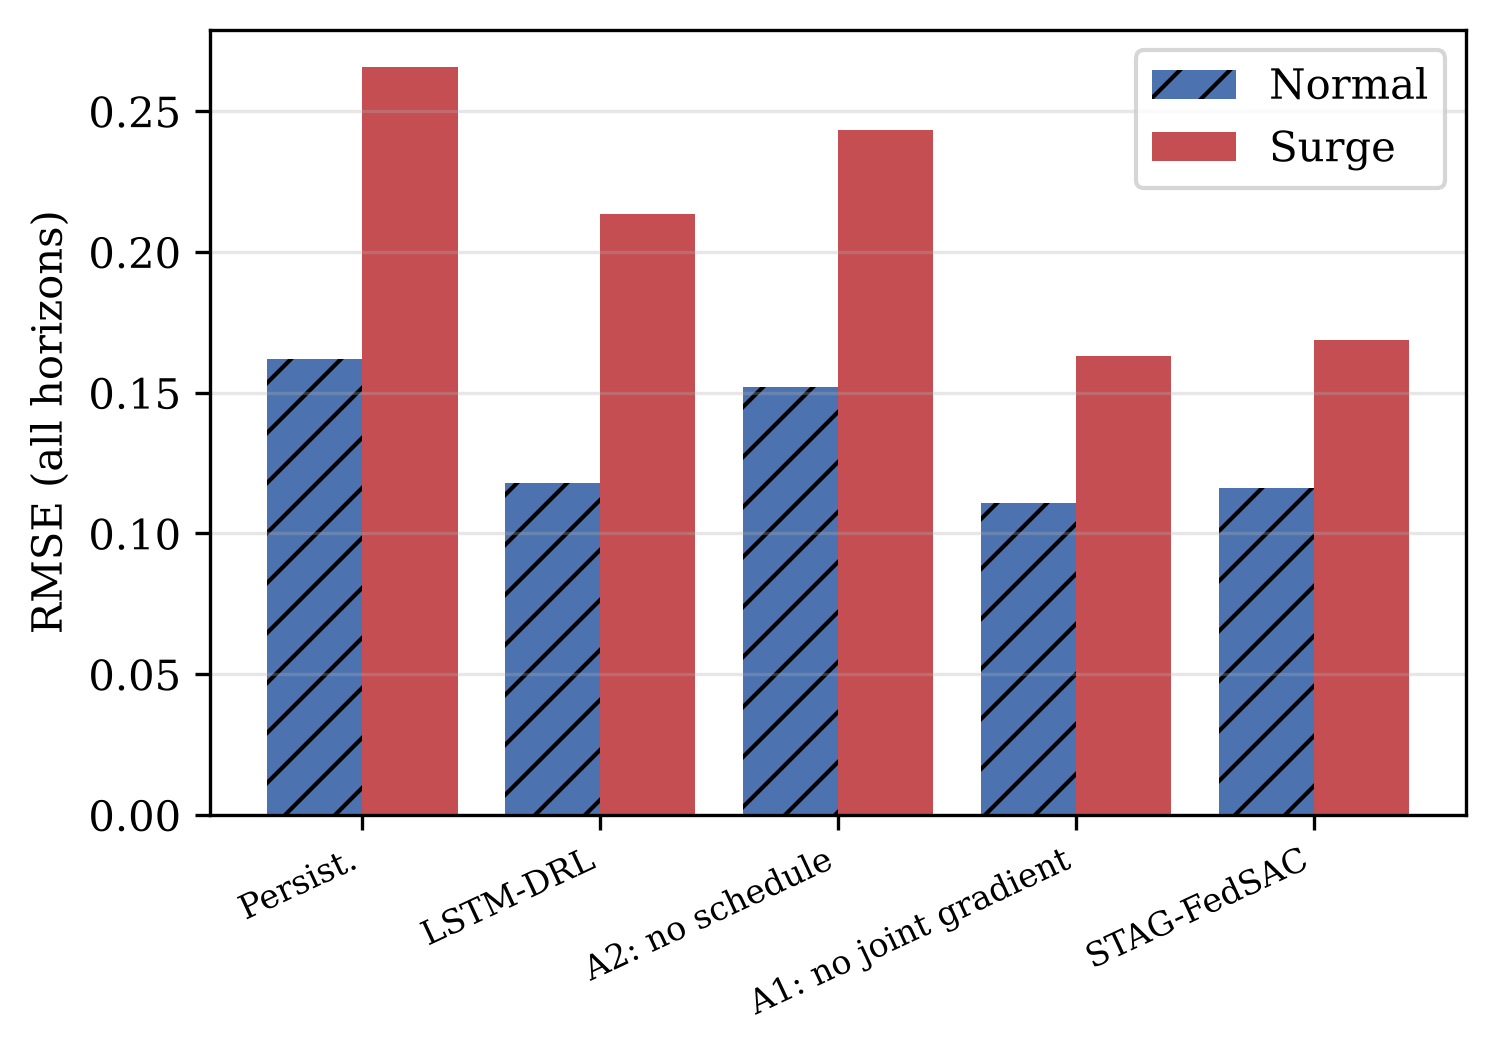
\includegraphics[width=0.6\linewidth]{fig_prediction.png}
\caption{Forecast RMSE on surge and non-surge AP/interval pairs.}
\label{fig:pred}
\end{figure}

\subsection{Ablation of the Contributions}
\label{sec:exp-abl}
To isolate the specific contributions of schedule conditioning, state representation design, and gradient coupling, we conduct systematic ablation studies (Tables~\ref{tab:main}, \ref{tab:pred}, and~\ref{tab:eta}).

\paragraph{Impact of Schedule Conditioning (Ablation A2)} 
Removing the transit schedule features from the predictor and the policy input degrades forecasting clearly and control less clearly. The forecast RMSE rises from $\mAOneRmse$ to $\mATwoRmse$ and the surge-window RMSE from $\mPropSurgeRmse$ to $\mATwoSurgeRmse$ (Table~\ref{tab:pred}). For control, the like-for-like comparison is with the latent-embedding configuration with $\eta=0.1$, which also uses the embedding: its reward falls from $\mFullReward$ to $\mATwoReward$ (about $9\%$) and its latency rises from $\mFullLat$~ms to $\mATwoLat$~ms ($7.8\%$), but with three seeds the reward difference is within seed variation (its 95\% interval includes zero). Against the proposed configuration the gap is larger (reward $\mPropReward$ to $\mATwoReward$, latency $\mPropLat$~ms to $\mATwoLat$~ms), but that comparison also changes the state representation. We read these results as evidence that the timetable carries information that the historical counters do not, for forecasting; for control the evidence is suggestive only.

\paragraph{State Representation Design: Direct Schedule Features vs.\ Latent Embeddings} 
We investigate how predictive schedule knowledge is best communicated to the DRL policy: via compact, explicit schedule features $\mathbf{S}_i^{t+1}\in\mathbb{R}^8$ versus the full high-dimensional spatio-temporal latent embedding $\mathbf{Z}_{\mathrm{fused}}\in\mathbb{R}^{768}$. The results suggest the following for our setting:
\begin{itemize}
  \item \textbf{Compact Direct Representation (Proposed STAG-FedSAC)}: Directly injecting the 8 normalized schedule features (event times, passenger counts, and surge indicators) into the SAC state provides a compact, stationary, and semantically invariant representation. Because these features depend only on the deterministic timetable, transitions stored in the off-policy replay buffer $\mathcal{B}_i$ remain valid across subsequent training iterations, which should favour stable Q-function estimation; this configuration gives the best control performance among the SAC variants ($\mPropReward$, latency $\mPropLat$~ms).
  \item \textbf{Latent Embedding Injection}: In contrast, passing the uncompressed 768-dimensional latent embedding $\mathbf{Z}_{\mathrm{fused}}$ into the policy state exposes off-policy training to \emph{representation staleness}. As the ST-GCAT predictor updates its parameters $\phi$ during training, historical transitions stored in the replay buffer contain stale representations generated by earlier model checkpoints. A plausible consequence is non-stationarity in the critic's value estimates; we did not test this directly (for instance by recomputing the embeddings of stored transitions). The observed reward is lower than with the compact representation: $\mAOneReward$ with $\eta=0$ (latency $\mAOneLat$~ms) and $\mFullReward$ with $\eta=0.1$ (latency $\mFullLat$~ms), against $\mPropReward$ ($\mPropLat$~ms).
\end{itemize}
In our experiments, compact schedule features worked better than concatenating the latent embedding; we did not test other ways of using the embedding.

\paragraph{Predictor--Policy Gradient Coupling ($\eta$ Sweep)} 
We examine the effect of the bidirectional joint gradient coupling weight $\eta$ in Eq.~\eqref{eq:joint}, which backpropagates the actor objective into the ST-GCAT predictor. Table~\ref{tab:eta} evaluates $\eta \in \{0, 0.01, 0.10\}$. Among the three values tested, the decoupled objective ($\eta=0$) gives the highest reward ($\mAOneReward$) and the lowest forecast error (RMSE $\mAOneRmse$, Surge-RMSE $\mAOneSurgeRmse$). Increasing the joint gradient weight to $\eta=0.01$ and $\eta=0.10$ lowers the control reward (to $\mEtaSmallFullReward$ and $\mFullReward$) and slightly worsens the forecast accuracy (RMSE $\mEtaSmallFullRmse$ and $\mFullRmse$). 

A plausible explanation, which we did not test, is that in off-policy learning the critic evaluates historical buffer samples while the actor objective changes the predictor, so that backpropagating the policy gradient into ST-GCAT perturbs the embeddings that the stored transitions were computed with. We could not show a benefit of the joint gradient at any of the three weights.

\begin{table}[htbp]
\centering
\caption{Sensitivity to the joint gradient coupling weight $\eta$ (mean $\pm$ standard deviation over seeds; $\eta=0$ corresponds to decoupled training).}
\label{tab:eta}
\small
\begin{tabular}{llcccc}
\toprule
$\eta$ & Seeds & Reward & Lat. (ms) & RMSE & Surge-RMSE \\
\midrule
0 & 3 & 0.176{\tiny$\pm$0.009} & 118.4{\tiny$\pm$9.8} & 0.121{\tiny$\pm$0.000} & 0.163{\tiny$\pm$0.009} \\
0.1 & 3 & 0.141{\tiny$\pm$0.008} & 170.6{\tiny$\pm$8.6} & 0.127{\tiny$\pm$0.000} & 0.169{\tiny$\pm$0.006} \\
\bottomrule
\end{tabular}

\end{table}


\subsection{What Does Federation Buy?}
\label{sec:exp-fed}

\begin{table}[htbp]
\centering
\caption{Federation schemes for the same agents. Traffic is measured during training, summed over all APs and rounds (MB); inter-zone traffic includes the reference states shipped for distillation.}
\label{tab:fed}
\small
\adjustbox{max width=\linewidth}{\begin{tabular}{llcccccc}
\toprule
Scheme & Seeds & Reward & Lat. (ms) & JFI & QoS sat. & Intra-zone (MB) & Inter-zone (MB) \\
\midrule
Isolated (no federation) & 2 & 0.121{\tiny$\pm$0.004} & 184.6{\tiny$\pm$2.8} & 0.935{\tiny$\pm$0.009} & 0.584{\tiny$\pm$0.015} & 0.0 & 0.0 \\
Flat FedAvg & 2 & 0.141{\tiny$\pm$0.006} & 162.8{\tiny$\pm$2.9} & 0.954{\tiny$\pm$0.002} & 0.615{\tiny$\pm$0.000} & 0.0 & 7778.3 \\
Zone FedAvg only & 2 & 0.132{\tiny$\pm$0.005} & 176.9{\tiny$\pm$9.0} & 0.946{\tiny$\pm$0.010} & 0.606{\tiny$\pm$0.021} & 7778.3 & 0.0 \\
Hier. FedAvg+FedProx (weights) & 2 & 0.146{\tiny$\pm$0.005} & 156.9{\tiny$\pm$9.3} & 0.959{\tiny$\pm$0.009} & 0.637{\tiny$\pm$0.010} & 7778.3 & 155.6 \\
HierFed-KD (Proposed distillation) & 3 & 0.141{\tiny$\pm$0.008} & 170.6{\tiny$\pm$8.6} & 0.952{\tiny$\pm$0.007} & 0.614{\tiny$\pm$0.017} & 7785.5 & 4.5 \\
Pooled experience (centralised) & 2 & 0.100{\tiny$\pm$0.013} & 213.0{\tiny$\pm$7.0} & 0.902{\tiny$\pm$0.028} & 0.534{\tiny$\pm$0.028} & 0.0 & 0.0 \\
\bottomrule
\end{tabular}
}
\end{table}

All federation variants share identical per-AP SAC agents, reward formulations, simulation environments, and random seeds, differing solely in how model parameters and knowledge are shared across the network hierarchy. All variants in this comparison use the latent-embedding configuration with $\eta=0.1$; the HierFed-KD row therefore corresponds to the ``Latent Emb., $\eta{=}0.1$'' row of Table~\ref{tab:main} (reward $\mFullReward$), not to the proposed configuration ($\mPropReward$). Table~\ref{tab:fed} and Figure~\ref{fig:fed} summarize their held-out evaluation performance alongside exact byte-level communication measurements collected across the entire training campaign.

\paragraph{Benefits of Federated Collaboration} 
Sharing learned representations across the network hierarchy provides clear performance benefits over isolated learning. Isolated agents operating without federation achieve a reward of $\mIsoReward$ and an average latency of $\mIsoLat$~ms. In contrast, all federated variants achieve higher rewards ($0.132$--$0.146$) and reduced latency ($156.9$--$176.9$~ms). By sharing base feature representations, federated APs benefit from the collective experience of neighbouring APs experiencing diverse congestion conditions, which suggests that sharing helps in this setting (two to three seeds per variant, so the differences among the federated variants are not resolved).

\paragraph{Failure of Monolithic Experience Pooling} 
To examine whether unconstrained centralized data pooling could serve as an empirical upper bound, we evaluate a centralized learner that samples transitions indiscriminately from a single pooled replay buffer across all APs. Crucially, this pooled-experience approach achieves a reward of only $\mCentralReward$ and an elevated latency of $\mCentralLat$~ms, which is worse than isolated learning (two seeds). Because individual APs occupy heterogeneous spatial positions with distinct channel assignments, local contention domains, and traffic mixes, naive experience pooling creates severe policy-distribution mismatch for each agent's critic. This suggests that, for AP-specific policies, pooling the transitions of other APs is not helpful; we did not test other pooling schemes.

\paragraph{Bandwidth Efficiency and Privacy Boundaries} 
While achieving competitive control performance, HierFed-KD provides dramatic communication reductions across the wide-area inter-zone network. Flat FedAvg requires exchanging full model weights directly with a central controller, consuming $\commWanFlat$~MB of wide-area traffic over training. Weight-based hierarchical federation reduces this to $\commWanAFive$~MB by aggregating models at zone controllers before global synchronization.

HierFed-KD slashes wide-area inter-zone communication to only $\commWanFull$~MB total ($\commRefMB$~MB for periodic public reference states and $\commOutMB$~MB for soft policy distributions). This is a measured $\commRatioAFive\times$ bandwidth reduction relative to weight-based hierarchical federation and a $\commRatioFlat\times$ reduction relative to flat FedAvg. Furthermore, because only soft policy distributions on an unlabelled public reference set are transmitted across administrative zones, HierFed-KD keeps local replay transitions and per-user identifiers at the AP and exchanges no model weights between zones; this is data minimisation, not a formal privacy guarantee, since distilled outputs can still leak information.


\subsection{Robustness to the Simulator Assumptions}
\label{sec:exp-robust}

\begin{table}[htbp]
\centering
\caption{Reward / latency (ms) of the same trained policies evaluated under different assumptions. A policy trained without contention (``w/o MAC'') or without switching cost is evaluated in the full simulator in the first column.}
\label{tab:robust}
\small
\adjustbox{max width=\linewidth}{\begin{tabular}{lcccc}
\toprule
Policy & Full MAC, 3 s outage & No contention & No switch cost & 10 s outage \\
\midrule
SSF (trained w/ MAC) & 0.181{\tiny$\pm$0.001} / 125{\tiny$\pm$2} & 0.222{\tiny$\pm$0.001} / 70{\tiny$\pm$1} & 0.184{\tiny$\pm$0.001} / 124{\tiny$\pm$2} & 0.177{\tiny$\pm$0.001} / 135{\tiny$\pm$2} \\
LLF (trained w/ MAC) & 0.156{\tiny$\pm$0.001} / 145{\tiny$\pm$2} & 0.179{\tiny$\pm$0.002} / 117{\tiny$\pm$3} & 0.159{\tiny$\pm$0.001} / 144{\tiny$\pm$2} & 0.152{\tiny$\pm$0.001} / 155{\tiny$\pm$2} \\
FedDDPG (trained w/ MAC) & 0.116{\tiny$\pm$0.004} / 185{\tiny$\pm$7} & 0.174{\tiny$\pm$0.002} / 106{\tiny$\pm$4} & 0.136{\tiny$\pm$0.004} / 176{\tiny$\pm$8} & 0.084{\tiny$\pm$0.003} / 270{\tiny$\pm$7} \\
STAG-FedSAC (trained w/ MAC) & 0.141{\tiny$\pm$0.008} / 171{\tiny$\pm$9} & 0.200{\tiny$\pm$0.005} / 93{\tiny$\pm$4} & 0.146{\tiny$\pm$0.007} / 168{\tiny$\pm$8} & 0.134{\tiny$\pm$0.008} / 190{\tiny$\pm$10} \\
\bottomrule
\end{tabular}
}
\end{table}

\paragraph{MAC contention} Evaluated without contention, the very same policies obtain a much lower latency: SSF $\mNoMacEvalSSFLat$~ms instead of $\mSSFLat$~ms and STAG-FedSAC $\mNoMacEvalFullLat$~ms instead of $\mFullLat$~ms, i.e.\ a factor of about $1.8$ in both cases, and a higher reward ($\mNoMacEvalFullReward$ against $\mFullReward$ for STAG-FedSAC). A simulator that ignores contention therefore understates latency by roughly 45\%, and the ``clean'' latency of the first version was an artefact of that omission. Policies that were \emph{trained} without contention and evaluated with it are clearly worse than policies trained with it (STAG-FedSAC $\mNoMacFullReward$ against $\mFullReward$; FedDDPG $\mNoMacFedDDPGReward$ against $\mFedDDPGReward$; two training seeds for the former), so contention-unaware planning is not only optimistic but also leads to worse configurations.

\paragraph{Channel-switching cost} Varying the outage in the evaluation from $0$ to $3$ to $10$~s changes the reward of STAG-FedSAC from $\mNoSwEvalFullReward$ to $\mFullReward$ to $\mSwTenEvalFullReward$, and its latency from $\mNoSwEvalFullLat$ to $\mFullLat$ to $\mSwTenEvalFullLat$~ms. The cost matters most for methods that switch often: FedDDPG, which changes the channel of about three quarters of the APs per interval, falls from $\mNoSwEvalFedDDPGReward$ to $\mSwTenEvalFedDDPGReward$ between $0$ and $10$~s, whereas SSF, which does not switch after the first interval, is almost unaffected. A policy trained without any switching cost and evaluated with the 3~s cost reaches $\mOutZeroFullReward$ against $\mFullReward$ for the policy trained with it (two seeds); this difference is within the seed-to-seed variation, so we cannot show that training with the cost helps.


\subsection{Sensitivity to the Reward Weights}
\label{sec:exp-weights}

\begin{table}[htbp]
\centering
\caption{Sensitivity to the reward weights (one training seed per cell; reward is computed with the weights used in training, so rewards are not comparable across rows; latency and JFI are).}
\label{tab:weights}
\small
\adjustbox{max width=\linewidth}{\begin{tabular}{lccccccccc}
\toprule
 & \multicolumn{3}{c}{SSF} & \multicolumn{3}{c}{FedDDPG} & \multicolumn{3}{c}{STAG-FedSAC} \\
\cmidrule(lr){2-4}\cmidrule(lr){5-7}\cmidrule(lr){8-10}
Weights ($\alpha/\beta/\gamma/\delta$) & Reward & Lat. & JFI & Reward & Lat. & JFI & Reward & Lat. & JFI \\
\midrule
Default (0.40/0.25/0.20/0.05) & 0.182 & 124 & 0.986 & 0.114 & 189 & 0.941 & 0.133 & 180 & 0.947 \\
Equal weights (0.25/0.25/0.25/0.25) & 0.106 & 124 & 0.986 & 0.046 & 165 & 0.935 & 0.059 & 166 & 0.952 \\
Throughput-heavy (0.55/0.15/0.20/0.10) & 0.308 & 124 & 0.986 & 0.226 & 196 & 0.928 & 0.250 & 188 & 0.942 \\
Latency-heavy (0.20/0.50/0.20/0.10) & -0.106 & 124 & 0.986 & -0.182 & 186 & 0.936 & -0.122 & 135 & 0.972 \\
\bottomrule
\end{tabular}
}
\end{table}

The reward weights are design choices (Section~\ref{sec:action}). To see whether the conclusions depend on them, we retrained STAG-FedSAC and FedDDPG with three other weightings and evaluated SSF with the same weights (Table~\ref{tab:weights}; the first row repeats the default weights for the same seed). The ordering of the methods is the same for all four weightings: SSF has the highest reward, STAG-FedSAC is second and FedDDPG third. STAG-FedSAC also has a higher JFI than FedDDPG in every row and a lower latency in three of the four rows (the equal-weights row is a tie within $2$~ms), the largest gap being under the latency-heavy weights. Each cell is a single training seed, so the table indicates robustness of the qualitative picture, not precise differences.

